% ------------------------------------------------------------------------------------
\section{Results}\label{sec:results}
\subsection{Main comparison}
Table~\ref{tab:main} and Fig.~\ref{fig:horizon} give test MAE, RMSE and MAPE on the June weeks, on exactly the Phase~1 samples. Four findings stand out.

\emph{(i) Deep sequence modelling alone already helps at longer horizons.} The GRU without any graph is worse than XGBoost-spatial at 15 minutes (\pMaeGRUFifteen{} vs \pMaeXGBsFifteen{}) but better at 30 and 60 minutes (\pMaeGRUSixty{} vs \pMaeXGBsSixty{}), although it sees no neighbour at all. A learned representation of the whole hour (level, slope, missingness, time) extrapolates further than 34 hand-built features.

\emph{(ii) The road graph adds a consistent gain on top.} With identical size and training, adding two graph-attention layers lowers MAE by \pRelGatVsGruFifteen\%, \pRelGatVsGruThirty\% and \pRelGatVsGruSixty\% at 15/30/60 minutes relative to the no-graph GRU; the fixed-weight diffusion model does the same. Against XGBoost-spatial, ST-GAT ties at 15 minutes (DM $p=\pDmPGATFifteen$) and is significantly better at 30 and 60 minutes (\pChgGATThirty\% and \pChgGATSixty\%, both $p<10^{-10}$) --- precisely the horizons at which the Phase~1 one-hop features faded.

\emph{(iii) Learned attention is not better than fixed road weights here.} DCRNN-lite (\pMaeGCNFifteen/\pMaeGCNThirty/\pMaeGCNSixty) and ST-GAT (\pMaeGATFifteen/\pMaeGATThirty/\pMaeGATSixty) are within a few hundredths of a mph, and the fixed-weight model is even slightly (but significantly) better at 30--60 minutes (\S\ref{sec:sig}). On a freeway graph whose links already encode driving distance, the Gaussian kernel is a good prior; attention earns its place through interpretability (\S\ref{sec:att}) rather than accuracy.

\emph{(iv) The hybrid is the best model at every horizon.} XGBoost + ST-GAT residual reaches \pMaeHybFifteen/\pMaeHybThirty/\pMaeHybSixty~mph, \pChgHybFifteen\%, \pChgHybThirty\% and \pChgHybSixty\% against XGBoost-spatial alone (DM statistics \pDmHybFifteen, \pDmHybThirty, \pDmHybSixty; all $p<10^{-10}$). Its biggest edge over the pure graph network is at 15 minutes (\pRelHybVsGatFifteen\%), where the tree model's sharp use of the current reading and the usual speed matters most; at 60 minutes the two converge, because there the correction carries most of the information. Each part does what it is best at: the tree model the per-sensor level and daily cycle, the graph network the propagation. For reference, DCRNN reports 2.77/3.15/3.60~\cite{li2018dcrnn} after 100 GPU epochs on a slightly different split; our CPU-trained hybrid is within 0.03--0.08~mph.

\begin{table*}[t]\centering
\caption{Test-set masked MAE, RMSE (mph) and MAPE (\%) by horizon, 4--27 June 2012, identical samples for all models. P1 = Phase~1 model, P2 = Phase~2. Best MAE in bold.}
\label{tab:main}\footnotesize\setlength{\tabcolsep}{4pt}
\begin{tabular}{llrrrrrrrrr}\hline
 & & \multicolumn{3}{c}{15 min} & \multicolumn{3}{c}{30 min} & \multicolumn{3}{c}{60 min}\\
Model & & MAE & RMSE & MAPE & MAE & RMSE & MAPE & MAE & RMSE & MAPE\\\hline
Historical average & P1 & 4.19 & 7.86 & 13.1 & 4.19 & 7.86 & 13.1 & 4.19 & 7.86 & 13.1\\
Persistence & P1 & 3.49 & 6.38 & 8.6 & 4.18 & 8.00 & 10.8 & 5.33 & 10.27 & 14.4\\
XGBoost + nbrs & P1 & 2.87 & 5.18 & 7.6 & 3.32 & 6.16 & 9.4 & 3.78 & 7.07 & 11.2\\
Random Forest + nbrs & P1 & 2.87 & 5.16 & 7.7 & 3.31 & 6.09 & 9.4 & 3.81 & 7.06 & 11.3\\
\hline
GRU, no graph & P2 & 2.91 & 5.71 & 8.0 & 3.31 & 6.68 & 9.6 & 3.71 & 7.69 & 11.4\\
Diffusion GCN & P2 & 2.88 & 5.51 & 7.7 & 3.24 & 6.41 & 9.1 & \textbf{3.66} & 7.44 & 10.9\\
ST-GAT & P2 & 2.88 & 5.52 & 7.9 & 3.26 & 6.46 & 9.5 & 3.68 & 7.52 & 11.3\\
ST-GAT + LWR & P2 & 2.88 & 5.53 & 7.9 & 3.25 & 6.46 & 9.4 & 3.68 & 7.50 & 11.2\\
Hybrid XGB+ST-GAT & P2 & \textbf{2.80} & 5.20 & 7.4 & \textbf{3.23} & 6.19 & 9.1 & 3.68 & 7.15 & 11.0\\
\hline\end{tabular}\end{table*}


\begin{figure}[t]\centering
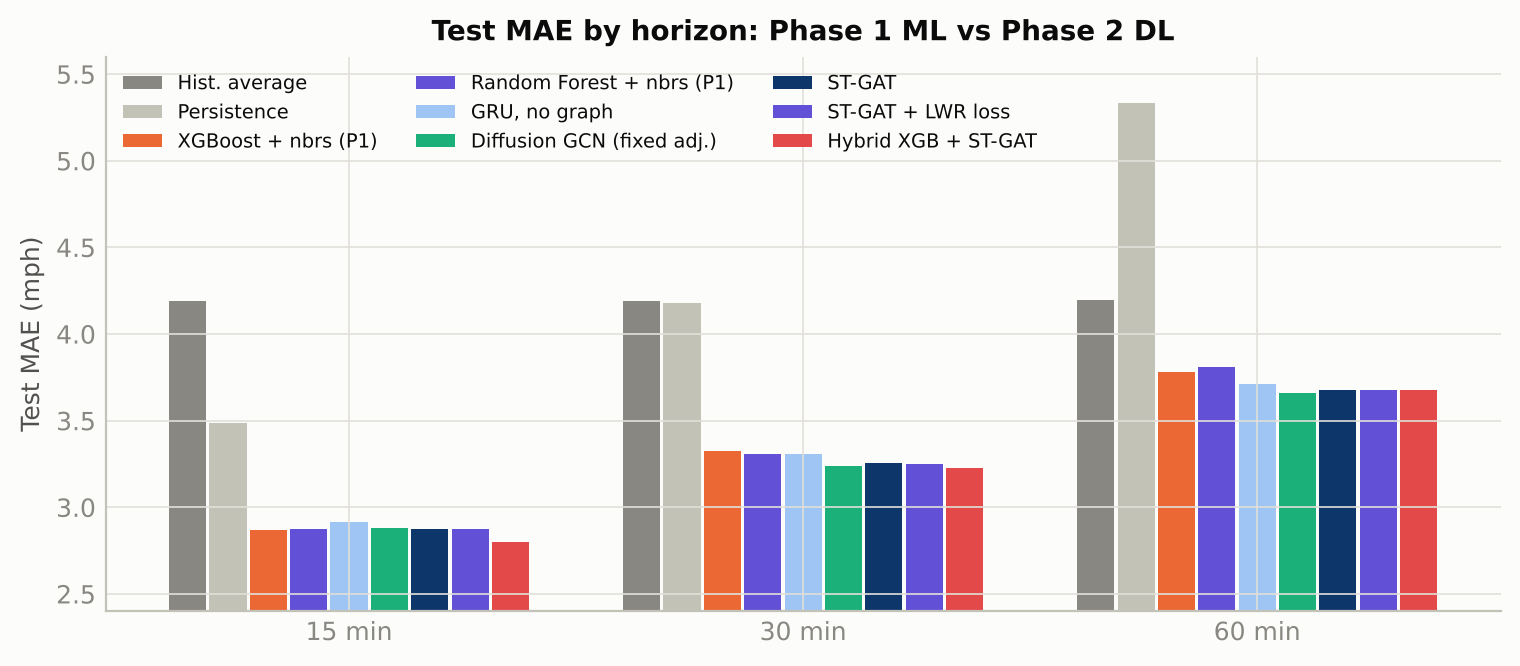
\includegraphics[width=\columnwidth]{fig_dl_mae_by_horizon}
\caption{Test MAE by horizon for the Phase~1 references and the Phase~2 models.}
\label{fig:horizon}
\end{figure}

\subsection{Rush hour}
Table~\ref{tab:peak} and Fig.~\ref{fig:gain} split the 60-minute errors by period. The graph models improve on XGBoost-spatial in both weekday rush hours and off-peak. In mph the gains are similar or slightly larger in the peaks (hybrid: \pPeakXGBsSixty{} $\rightarrow$ \pPeakHybSixty{} peak, \pOffXGBsSixty{} $\rightarrow$ \pOffHybSixty{} off-peak); in relative terms they are slightly larger off-peak (\pChgPeakHybSixty\% vs \pChgOffHybSixty\%), because the off-peak error is small to begin with. The no-graph GRU gains almost nothing in the peaks (\pChgPeakGRUSixty\%) while the diffusion model gains \pChgPeakGCNSixty\%: in rush hour the improvement comes from the graph. Rush hour remains about 1.7$\times$ harder than off-peak for every model; it is still where most of the error is. The congestion map (Fig.~\ref{fig:map}) shows the evening jam of 13~June as forecast an hour ahead.

\begin{table}[t]\centering
\caption{Test MAE (mph) at 60 minutes, weekday rush hours (07--10, 16--19) vs off-peak, and change vs XGBoost-spatial.}
\label{tab:peak}\footnotesize
\begin{tabular}{lrrrr}\hline
Model & Peak & $\Delta$ & Off-peak & $\Delta$\\\hline
XGBoost + nbrs & 5.67 & -- & 3.31 & --\\
GRU, no graph & 5.67 & +0.1\% & 3.22 & -2.7\%\\
Diffusion GCN & 5.54 & -2.2\% & 3.18 & -3.8\%\\
ST-GAT & 5.62 & -0.8\% & 3.19 & -3.6\%\\
ST-GAT + LWR & 5.63 & -0.6\% & 3.18 & -3.7\%\\
Hybrid XGB+ST-GAT & 5.53 & -2.3\% & 3.21 & -3.0\%\\
\hline\end{tabular}\end{table}


\begin{figure*}[t]\centering
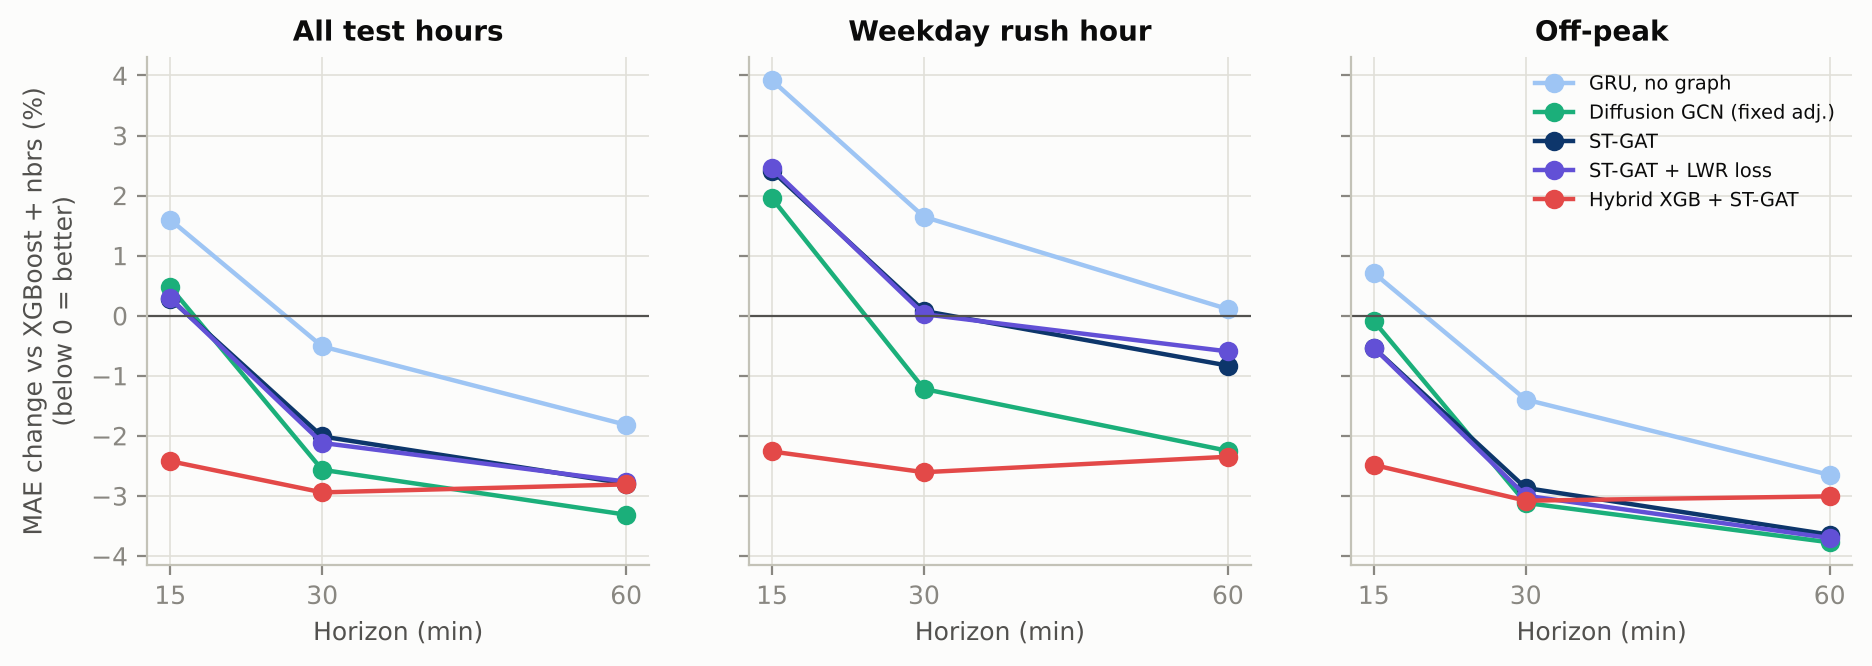
\includegraphics[width=0.95\textwidth]{fig_dl_gain_vs_xgb}
\caption{MAE change of each Phase~2 model relative to XGBoost-spatial (Phase~1's best), overall, in weekday rush hours and off-peak. Below zero is better.}
\label{fig:gain}
\end{figure*}

\begin{figure*}[t]\centering
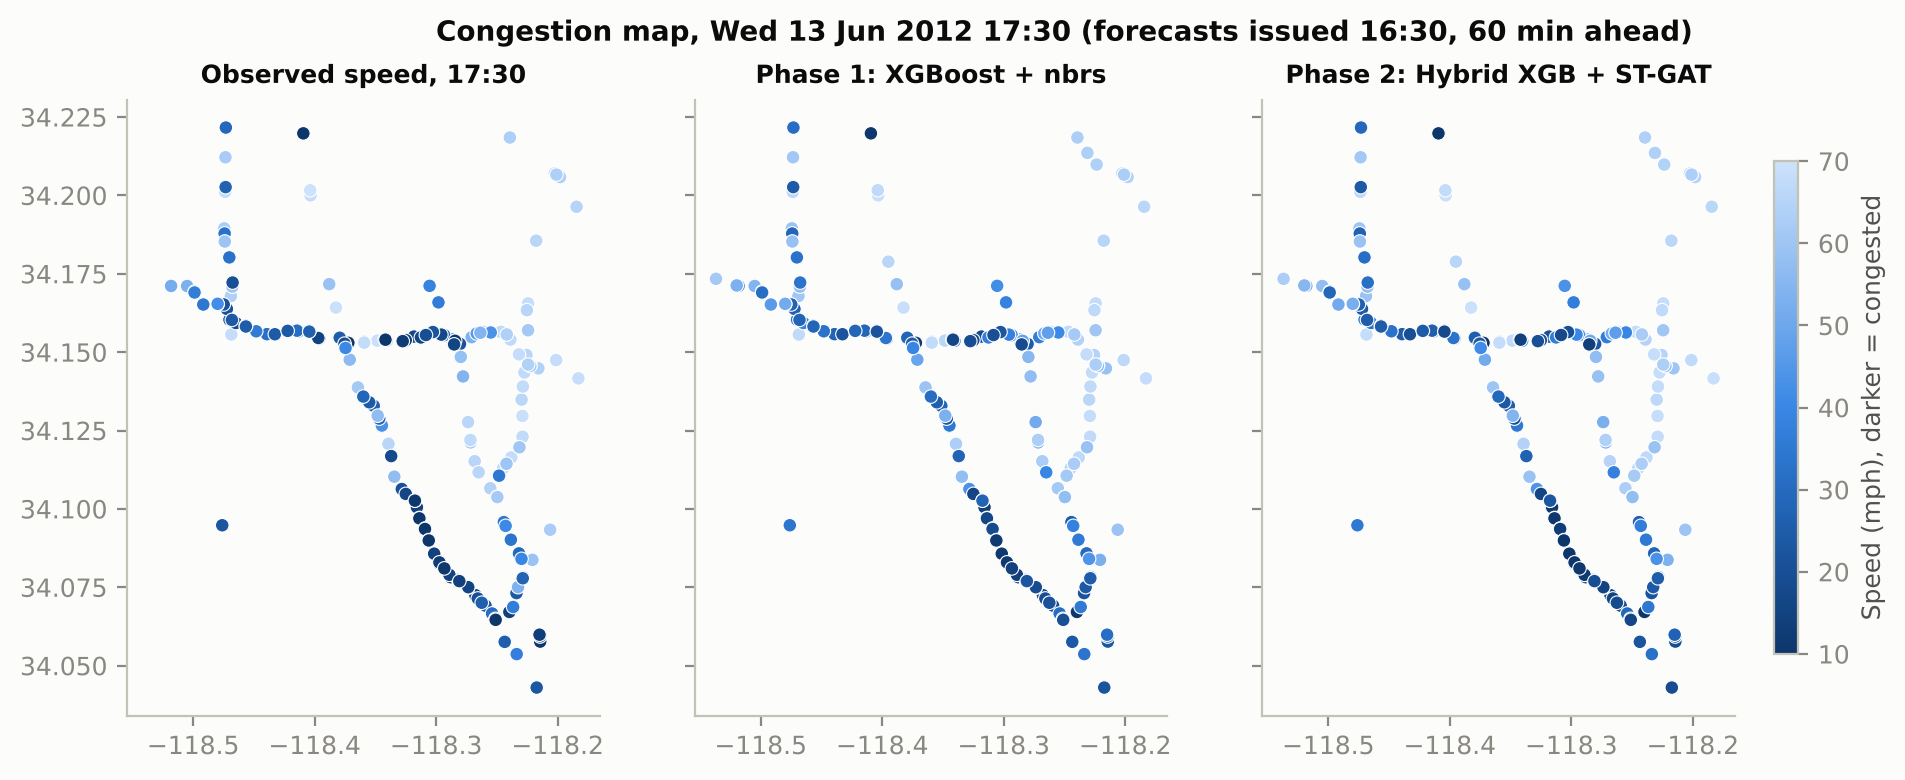
\includegraphics[width=0.95\textwidth]{fig_dl_congestion_map}
\caption{Congestion map, Wednesday 13 June 2012 at 17:30: observed speeds and 60-minute-ahead forecasts from XGBoost-spatial and the best Phase~2 model.}
\label{fig:map}
\end{figure*}

\subsection{Jam detection and large errors}
Scored as a detector of speeds below 35~mph at 60 minutes, the graph models catch more jams than XGBoost-spatial: recall rises from \pRecXGBsSixty{} to \pRecGCNSixty{} (diffusion) and \pRecGATSixty{} (ST-GAT), F1 from \pFoneXGBsSixty{} to \pFoneGCNSixty{} and \pFoneGATSixty, at a small cost in precision. The pure deep models, however, have a \emph{higher RMSE} than XGBoost (\pRmseGATSixty{} vs \pRmseXGBsSixty{} at 60 minutes): trained on absolute error, they predict something close to the conditional median and under-predict the rare, deep speed drops that dominate squared error. The hybrid, anchored on the tree forecast, keeps RMSE close to XGBoost's (\pRmseHybSixty) while improving MAE. A Huber or quantile loss is the natural next step.

\subsection{Is each difference real?}\label{sec:sig}
Table~\ref{tab:dmpairs} applies the Diebold--Mariano test to the key pairs. Adding the graph to the same network is significant at every horizon (ST-GAT vs GRU: DM $=-12.6,-11.4,-4.8$; diffusion vs GRU: $-9.1,-12.4,-6.1$), and so is adding it inside the hybrid (hybrid vs hybrid without graph: $-14.6,-13.2,-11.4$). Attention vs fixed weights goes the other way at 30--60 minutes: the diffusion model is slightly but significantly better ($p<0.01$). The LWR penalty makes no significant difference at any horizon ($p\geq0.09$). The hybrid beats pure ST-GAT at 15 and 30 minutes and ties at 60 ($p=0.96$). These tests treat each trained model as fixed; they do not include run-to-run variation, which we estimate below.

\begin{table}[t]\centering
\caption{Diebold--Mariano statistics for key pairs (negative = first model more accurate), test weeks.}
\label{tab:dmpairs}\footnotesize
\begin{tabular}{lrrr}\hline
Pair & 15 min & 30 min & 60 min\\\hline
ST-GAT vs GRU (no graph) & $-12.6$ & $-11.4$ & $-4.8$\\
Diffusion vs GRU (no graph) & $-9.1$ & $-12.4$ & $-6.1$\\
ST-GAT vs Diffusion & $-2.0$ & $+4.5$ & $+2.8$\\
Hybrid vs hybrid without graph & $-14.6$ & $-13.2$ & $-11.4$\\
Hybrid vs ST-GAT & $-16.4$ & $-4.2$ & $-0.1$\\
ST-GAT+LWR vs ST-GAT & $+0.2$ & $-1.7$ & $+0.3$\\
Hybrid vs XGBoost-spatial & \pDmHybFifteen & \pDmHybThirty & \pDmHybSixty\\
\hline\end{tabular}\end{table}

\subsection{Ablations and seeds}
Table~\ref{tab:abl} and Fig.~\ref{fig:abl} report the design ablations under the identical 12-epoch budget. Three seeds of the reference model give \pSeedMeanFifteen~$\pm$~\pSeedStdFifteen{} mph at 15 minutes and \pSeedMeanSixty~$\pm$~\pSeedStdSixty{} mph at 60 minutes; the reference run (seed 42, \pMaeShortSixty{} at 60 minutes) happens to be the weakest of the three, so differences should be read against this spread. Read that way:
\begin{itemize}
\item \textbf{Hops:} 3 layers reach \pMaeThreeHopSixty{} at 60 minutes, about one seed standard deviation better than 2 layers on average, while 1 layer (\pMaeOneHopSixty) is no better than 2 --- weak evidence, consistent with the LWR argument, that more hops help the longest horizon.
\item \textbf{Graph structure, direction and masking} (random graph \pMaeRandSixty, undirected \pMaeUndirSixty, outages as 0~mph \pMaeZeroSixty{} at 60 minutes) stay within the seed spread under this short budget; the masked model is better at 15 minutes (\pMaeShortFifteen{} vs \pMaeZeroFifteen). Twelve epochs are not enough for the network to exploit the road structure fully; the full-budget, significance-tested comparisons above are the evidence that the graph matters.
\item \textbf{Regularisation:} switching off dropout and weight decay \emph{helps} under the short budget (\pMaeNoDropSixty{} at 60 minutes): with few epochs the model under-fits, and regularisation slows it down further. This is the expected behaviour early in training and is why the main models use early stopping over a longer budget rather than a fixed short one.
\item \textbf{Hybrid without graph} (\pMaeHybNoFifteen/\pMaeHybNoThirty/\pMaeHybNoSixty) is already strong, and the graph version improves on it significantly at every horizon.
\end{itemize}

\begin{table}[t]\centering
\caption{Ablations under an identical 12-epoch budget: test MAE (mph) and change vs the reference ST-GAT-short.}
\label{tab:abl}\footnotesize
\begin{tabular}{lrrrr}\hline
Variant & 15 min & 60 min & $\Delta$15 & $\Delta$60\\\hline
reference (2 hops) & 3.00 & 4.08 & -- & --\\
1 hop & 3.00 & 4.09 & +0.001 & +0.008\\
3 hops & 2.98 & 3.97 & -0.017 & -0.104\\
undirected edges & 2.98 & 4.03 & -0.015 & -0.045\\
random graph & 2.99 & 4.08 & -0.010 & -0.003\\
outages as 0 mph & 3.03 & 4.09 & +0.036 & +0.008\\
no dropout/decay & 2.95 & 3.93 & -0.046 & -0.151\\
hybrid, no graph & 2.81 & 3.70 & -0.191 & -0.381\\
\hline\end{tabular}\end{table}


\begin{figure}[t]\centering
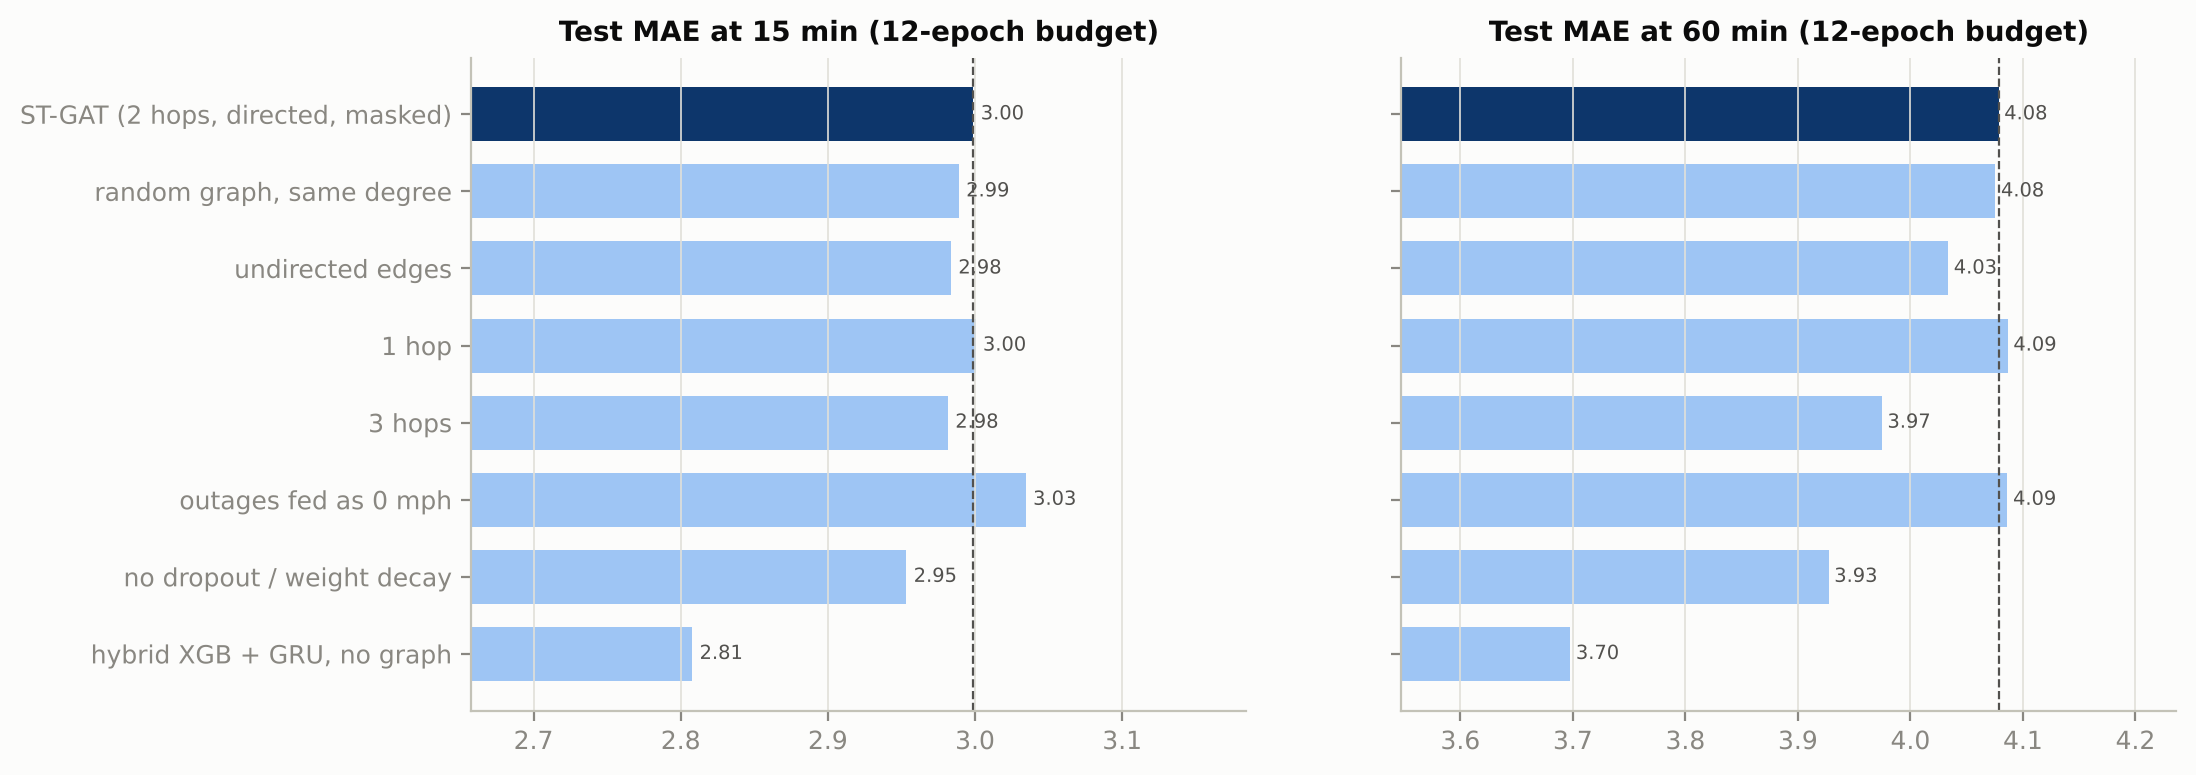
\includegraphics[width=\columnwidth]{fig_dl_ablations}
\caption{Ablations under the same 12-epoch budget; dashed line = reference ST-GAT-short.}
\label{fig:abl}
\end{figure}


\subsection{Where the attention looks}\label{sec:att}
In the undirected ST-GAT one softmax covers a sensor itself and both its upstream and downstream neighbours, so attention shares can be compared (Fig.~\ref{fig:att}). When a sensor is free-flowing it puts \pAttFreeSelf\% of its first-layer attention on itself, \pAttFreeDownstream\% on downstream and \pAttFreeUpstream\% on upstream neighbours; when it is jammed the shares become \pAttJammedSelf\%, \pAttJammedDownstream\% and \pAttJammedUpstream\%. This is an analysis of one trained model and one layer, not a causal statement, but it is the kind of check that relates what the network learned to the LWR picture of queues and platoons.

\begin{figure}[t]\centering
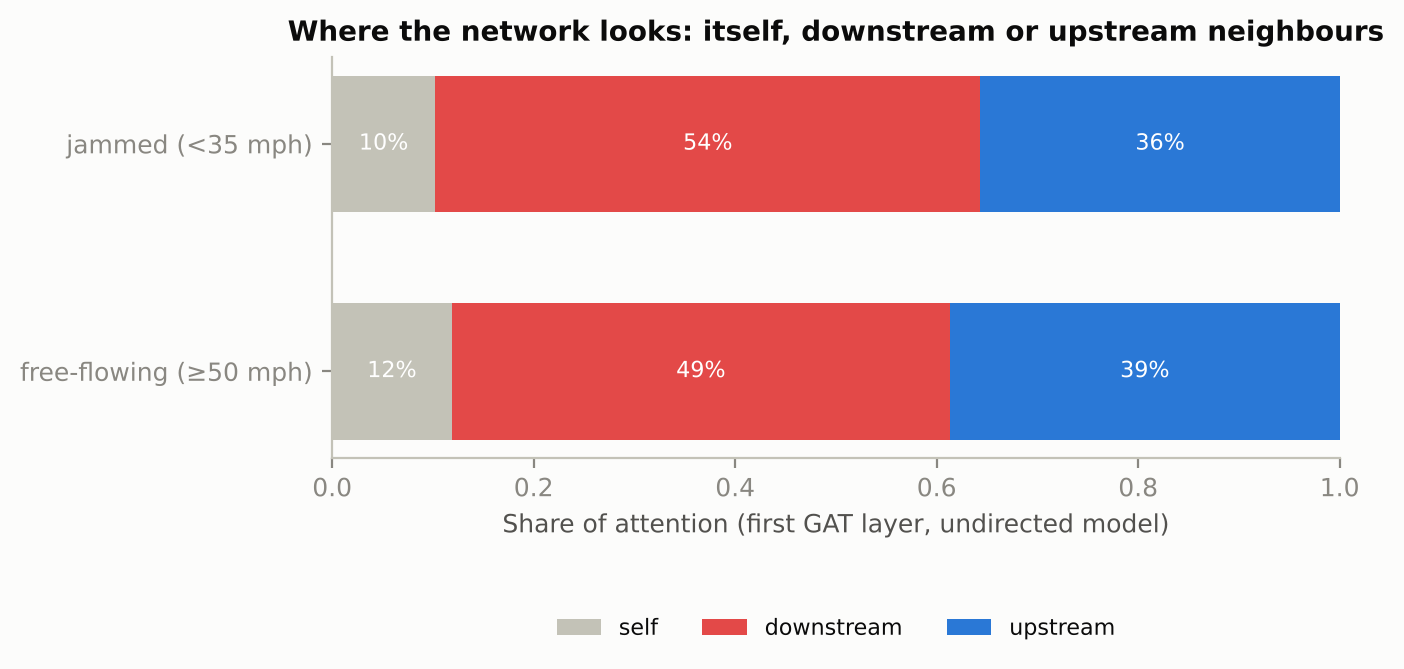
\includegraphics[width=\columnwidth]{fig_dl_attention}
\caption{Share of first-layer attention placed on the sensor itself, its downstream and its upstream neighbours (undirected ST-GAT, 1{,}500 random test times), for free-flowing vs jammed sensors.}
\label{fig:att}
\end{figure}
